\documentclass{standalone}
\usepackage{tikz}
\usetikzlibrary{patterns, angles}

\begin{document}
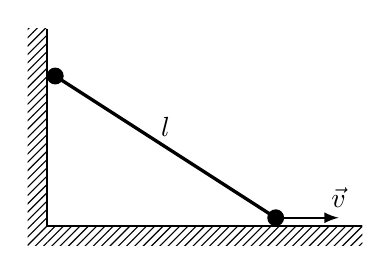
\begin{tikzpicture}
	\coordinate (A) at (0, 2);
    \coordinate (C) at (0, 2.5);
    \coordinate (O) at (0, 0);
    \coordinate (D) at (4, 0);
    \coordinate (B) at (3, 0);
    \coordinate (M) at (1.5, 1);
       
	\draw [draw=none, pattern=north east lines] (C) rectangle (-0.25,-0.25);
	\draw [draw=none, pattern=north east lines] (0,-0.25) rectangle (D);	
	\draw [thick] (C) -- (O) -- (D);
	\draw [very thick] (0.1,1.9) -- (2.9,0.1) node [midway, above] {$l$};
	\draw [fill] (0.1,1.9) circle (0.1);	
	\draw [fill] (2.9,0.1) circle (0.1);
	%\pic [draw, -, angle eccentricity=1.5] {angle = O--A--B};
	%\node [right=10pt, below=10pt] at (A) {$\alpha$};
	\draw [arrows={-latex}, thick] (3,0.1) -- (3.7, 0.1) node [above]  {$\vec{v}$};
\end{tikzpicture}
\end{document}